\section{Preliminares}\label{sec:prelim}

En esta sección se presenta una breve descripción de los conceptos fundamentales
más importantes para hacer posible la comprensión y discusión sobre las
contribuciones de este trabajo.

\subsection{Sistemas distribuídos}
\subsubsection{El problema de los generales bizantinos}

\subsection{Los orígenes de la blockchain}
Las blockchains tomaron popularidad con la invención de Bitcoin en 2008, luego de la publicación
de un artículo llamado \textit{Bitcoin: A Peer-to-Peer
Electronic Cash System}\footnote{Bitcoin: un sistema de dinero electrónico de par a par.}, escrito
bajo el pseudónimo de Satoshi Nakamoto.
Nakamoto combinó diversas invenciones previas como
\textit{b-money} y \textit{HashCash} para crear un sistema de dinero electrónico completamente
descentralizado que, justamente, no necesita confiar en ninguna autoridad central para la emisión de monedas,
o la liquidación o validación de las transacciones. 
La innovación clave en Bitcoin fue el uso de un sistema de cómputo distribuído que lleva
a cabo una elección global de las nuevas transacciones cada 10 minutos, permitiendo
a la red descentralizada llegar a un consenso sobre el estado de las mismas. Estas transacciones
se guardan empaquetadas como bloques en una bitácora distribuída pública conocida como blockchain.
Se dice que estas transacciones se encuentran totalmente ordenadas porque es posible determinar para
dos transacciones cualesquieras en la blockchain cuál de ellas ocurrió antes.

%Esto resolvió de forma elegante el problema del doble gasto,
%en el cual una misma unidad de moneda se utiliza dos veces. Previamente, el problema del doble gasto fue
%una debilidad de los sistemas de moneda digital que fue abordado mediante servidores de información centrales.

Bitcoin es una colección de conceptos y tecnologías que forman las bases de un ecosistema de dinero
digital. Si bien la noción de bitcoin como criptomoneda no es imprescindible para la comprensión de las
contribuciones de este trabajo, es el primer caso de uso que da particular importancia a la blockchain
como tal y a su rendimiento. Por este motivo se considera pertinente presentar un breve resumen sobre
su funcionamiento.

\subsubsection{Funcionamiento de bitcoin}

Las unidades de moneda llamadas bitcoins son usadas para almacenar y transmitir valor a través
de los participantes de la red de bitcoin. Los usuarios se comunican entre ellos usando un protocolo 
específico principalmente mediante internet. La pila del
protocolo bitcoin, disponible como software de código abierto, se puede correr en una amplia gama de
dispositivos, incluyendo computadoras portátiles y teléfonos inteligentes, haciéndolo una tecnología
fácilmente accesible.

Los usuarios pueden transferir bitcoins en la red y hacer básicamente cualquier operación que puede ser
realizada con monedas tradicionales, incluyendo comprar y vender bienes, enviar dinero a personas u
organizaciones, o extender créditos. Los bitcoins también pueden ser vendidos, comprados, o intercambiados por
otras monedas en casas de cambio especializadas.

A diferencia de las monedas tradicionales, los bitcoins son completamente virtuales. No hay monedas
físicas e incluso no existen monedas en sí. Las monedas se representan en transacciones que transfieren
valor desde el remitente hacia el destinatario. Los usuarios de bitcoin poseen claves criptográficas
que permiten probar la propiedad de los bitcoins en la red. Con estas claves se pueden firmar las
transacciones para desbloquear el valor y utilizarlo transfiriéndolo a un nuevo dueño. 
%Las claves
%son a menudo guardadas en billeteras digitales en las computadoras o celulares de los usuarios. La
%posesión de una clave que puede firmar una transacción es el único prerequisito para utilizar bitcoin,
%poniendo el control enteramente en manos de cada usuario.

Bitcoin es un sistema distribuído de par a par. Como tal no tiene un servidor central o un punto de control.
Los bitcoins son creados a través de un proceso llamado \textit{minería}, el cual involucra una competencia
para encontrar solución a un problema matemático mientras se procesan las transacciones de bitcoin.
Cualquier participante de la red (es decir, cualquiera quien use un dispositivo que corre la pila
completa de protocolo de bitcoin) puede operar como minero, usando el poder de procesamiento de su
computadora para verificar y guardar transacciones. Cada 10 minutos, en promedio, alguien logra validar
las transacciones de los últimos 10 minutos y es compensando con bitcoin nuevo. Esencialmente, la minería
de bitcoins descentraliza la emisión de moneda y las funciones de compensación de un banco central, evitando
la necesidad del mismo.

El protocolo de bitcoin incluye algoritmos nativos que regulan las funciones de minería a lo largo de la
red. La dificultad de la tarea de procesamiento que los mineros deben realizar se ajusta dinámicamente
de modo que, en promedio, alguien tiene éxito cada 10 minutos sin importar la cantidad de mineros (y
de poder de cómputo) existente en un momento dado. El protocolo además disminuye a la mitad el ratio de creación
de bitcoins cada 4 años, y limita el número total de bitcoins que serán creados a un número fijo de
aproximadamente 21 millones de bitcoins.

%El resultado es que el número de bitcoins en circulación
%sigue una curva predecible fácilmente que llega a 21 millones para el 2140. Debido a la disminución de
%emisión de bitcoins, a largo plazo, el bitcoin es deflacionario. Incluso más, bitcoin no puede sufrir
%inflación por "imprimir" más dinero más allá de ratio esperado. 

%Detrás de escena, bitcoin es el nombre de un protocolo, una red de pares, y una innovación de
%computación distribuída.
Bitcdoin representa la culminación de décadas de investigación en criptografía
y sistemas distribuídos, e incluye 4 innovaciones claves funcionando juntas:
\begin{itemize}
  \item Una red de par a par descentralizada (el protocolo de bitcoin)
  \item Una bitácora distribuída pública de transacciones organizadas en bloques (la blockchain)
  \item Un conjunto de reglas para la validación independiente de transacciones y la emisión de monedas (reglas de consenso)
  \item Un mecanismo para lograr un consenso global descentralizado en la blockchain (algoritmo de prueba de trabajo)
\end{itemize}

\subsubsection{La forma de la blockchain}

Cada nodo completo en la red de bitcoin guarda independientemente una blockchain que contiene solo
bloques validados por ese nodo. Cuando cierta cantidad de nodos tienen los mismos bloques en su propia blockchain
se dice que llegaron a un consenso. 
%The validation rules these nodes follow to maintain consensus are
%called consensus rules. This section describes many of the consensus rules used by Bitcoin Core.

La Figura muestra una versión simplificada de una blockchain. En la sección de datos de un bloque
se agrupan y alojan una o más transacciones nuevas. Copias de cada transacción se hashean, los hashes luego
se emparejan, se hashean, se emparejan de nuevo, y se hashean hasta que queda un único hash: la raíz de un
\textit{merkle tree}. 

La raíz del merkle tree se aloja en el encabezado del bloque. Cada bloque además contiene el hash del encabezado
del bloque anterior, encadenándolos. Esto asegura que una transacción no pueda modificarse sin modificar el bloque
que la contiene y todos los bloques siguientes.

% Agregar imágenes de blockchain y de merkle tree.

%Las transacciones también están encadenadas. Es decir, cada transacción gasta los \textit{satoshis}\footnote{
%Satoshi es la unidad mínima de Bitcoin, llamada así por el pseudónimo de su creador, Satoshi Nakamoto. Un bitcoin
%es equivalente a 100 millones de Satoshis.} previamente recibidos en una o más transacciones previas, por lo
%que la entrada de una transacción es la salida de una transacción previa.

%\subsection{Blockchain actuales}


\subsection{Setchain}
\setchain \cite{Capretto.2022.Setchain} is a distributed concurrent data-type
that implements Byzantine tolerant distributed grown-only sets with barriers
(called epochs).
%
Barriers impose an order between elements in different epochs but not with
elements in the same epoch.
%
Therefore, \setchain relaxes the total order requirement imposed by blockchains,
and thus, can achieve higher throughput and scalability.
%
\setchain can be used for those applications, like digital
registries, where different elements in the blockchain need not be
ordered except across infrequent barriers.

\paragraph*{Setchain API.}
%
Let \(U\) be a set of elements that client processes can inject into the
\setchain.
%
Moreover, let \isValidElement\ be a function that nodes can use to locally
validate elements in \(U\).
%
A \setchain is a distributed data structure where a collection of server nodes
maintain:
% \begin{compactitem}
\begin{itemize}
\item a set $\<theset> \subseteq U$ of elements added;
\item a natural number $\<epoch> \in \mathbb{N}$;
\item a map $\<history> : [1..\<epoch>] \rightarrow \mathcal{P}(U)$\footnote{$\mathcal{P}(U)$ denotes the
power set of $U$} describing sets of elements that have been stamped with an
epoch number.
\end{itemize}
%
Server nodes support two operations: \(\<add>\) and \(\<get>\).
%
Operation \(\<add>\) requests to add an element, while operation \(\<get>\)
returns the values maintained by the node~(\(\<theset>,\<history>,\<epoch>\)).
%
We use dot-notation to invoke these operations, let \(v\) be a server node and
\(e\) an element: \(v.\<add>(e),v.\<get>\).

% Each server node $v$ supports two operations,
% available to any client process:
% % \begin{compactitem}
% \begin{itemize}
% \item $v.\<add>(e)$: requests to add $e$ to $\<theset>$.
% \item $v.\<get>()$: returns the values of $\<theset>$, $\<history>$,
%   and $\<epoch>$, as perceived by $v$.
% \end{itemize}

When barriers are triggered, nodes maintaining the \setchain collaboratively
decide which added elements are stamped with the current epoch and increase the
epoch number.
%
We call these events \emph{epoch increments}.
%
We assume that periodic synchronization barriers are triggered.

A typical workflow from the point of the view of a client is as follows: a
client invokes $\<add>(e)$ in one (or more) servers to insert a new valid
element $e$ in the \setchain.
%
The element $e$ will be propagated among the servers, and when an
epoch increment occurs, the servers will attempt to include it in the
new epoch.
%
After waiting for some time, the client invokes $\<get>$ in one (or
more) servers to check that the element has been effectively added and
stamped.

\paragraph*{Properties.}
To ensure correctness, \setchain implementations must satisfy certain
properties that provide eventual guarantees for elements added and
guarantee consistency between correct servers. 
%
These properties reason about correct servers since Byzantine servers
do not provide any guarantee.

\begin{compactitem}
  \item Every valid element added by a correct
server is eventually returned in all future gets issued in all correct
servers.
  \item All valid elements added in a correct server must be eventually
be stamped in all correct servers.
  \item Once an element is stamped with an epoch, it cannot be unstamped, nor
can it be stamped with another epoch.
\item Any two correct servers agree on the content of
all epochs that both have computed~\footnote{Not all correct servers process epoch increments
simultaneously, as some may be more delayed than others.}.
%
% Nevertheless,
\item Every element that is stamped comes from the result of a client adding the element.
  \end{compactitem}
\gabina{Epoch proofs are part of the epoch but are not coming directly from the result of a client adding element.}

\subsection{Tendermint}\label{sec:tendermint}
%
Tendermint is a state machine replication engine that tolerates Byzantine faults.
%
It was among the first systems to adapt classical Byzantine Fault Tolerant consensus protocols
to the blockchain paradigm, whereby consensus is performed on cryptographic hash-linked batches of
transactions (i.e., blocks) in a public, open-membership network.
%
Tendermint functions as a blockchain middleware that supports the replication of arbitrary
applications, written in any programming language~\cite{tendermint.design}.

In Figure~\ref{fig:replication}, we show the overview of replicated state machine architecture.
%
A replicated state machine replicates a transaction log and resulting state across multiple machines.
%
Transactions are received from the client, run through the consensus protocol, ordered in the
transaction log, and executed against the state.
%
% In the figure, each , with .
%

\begin{figure}
  \centering
  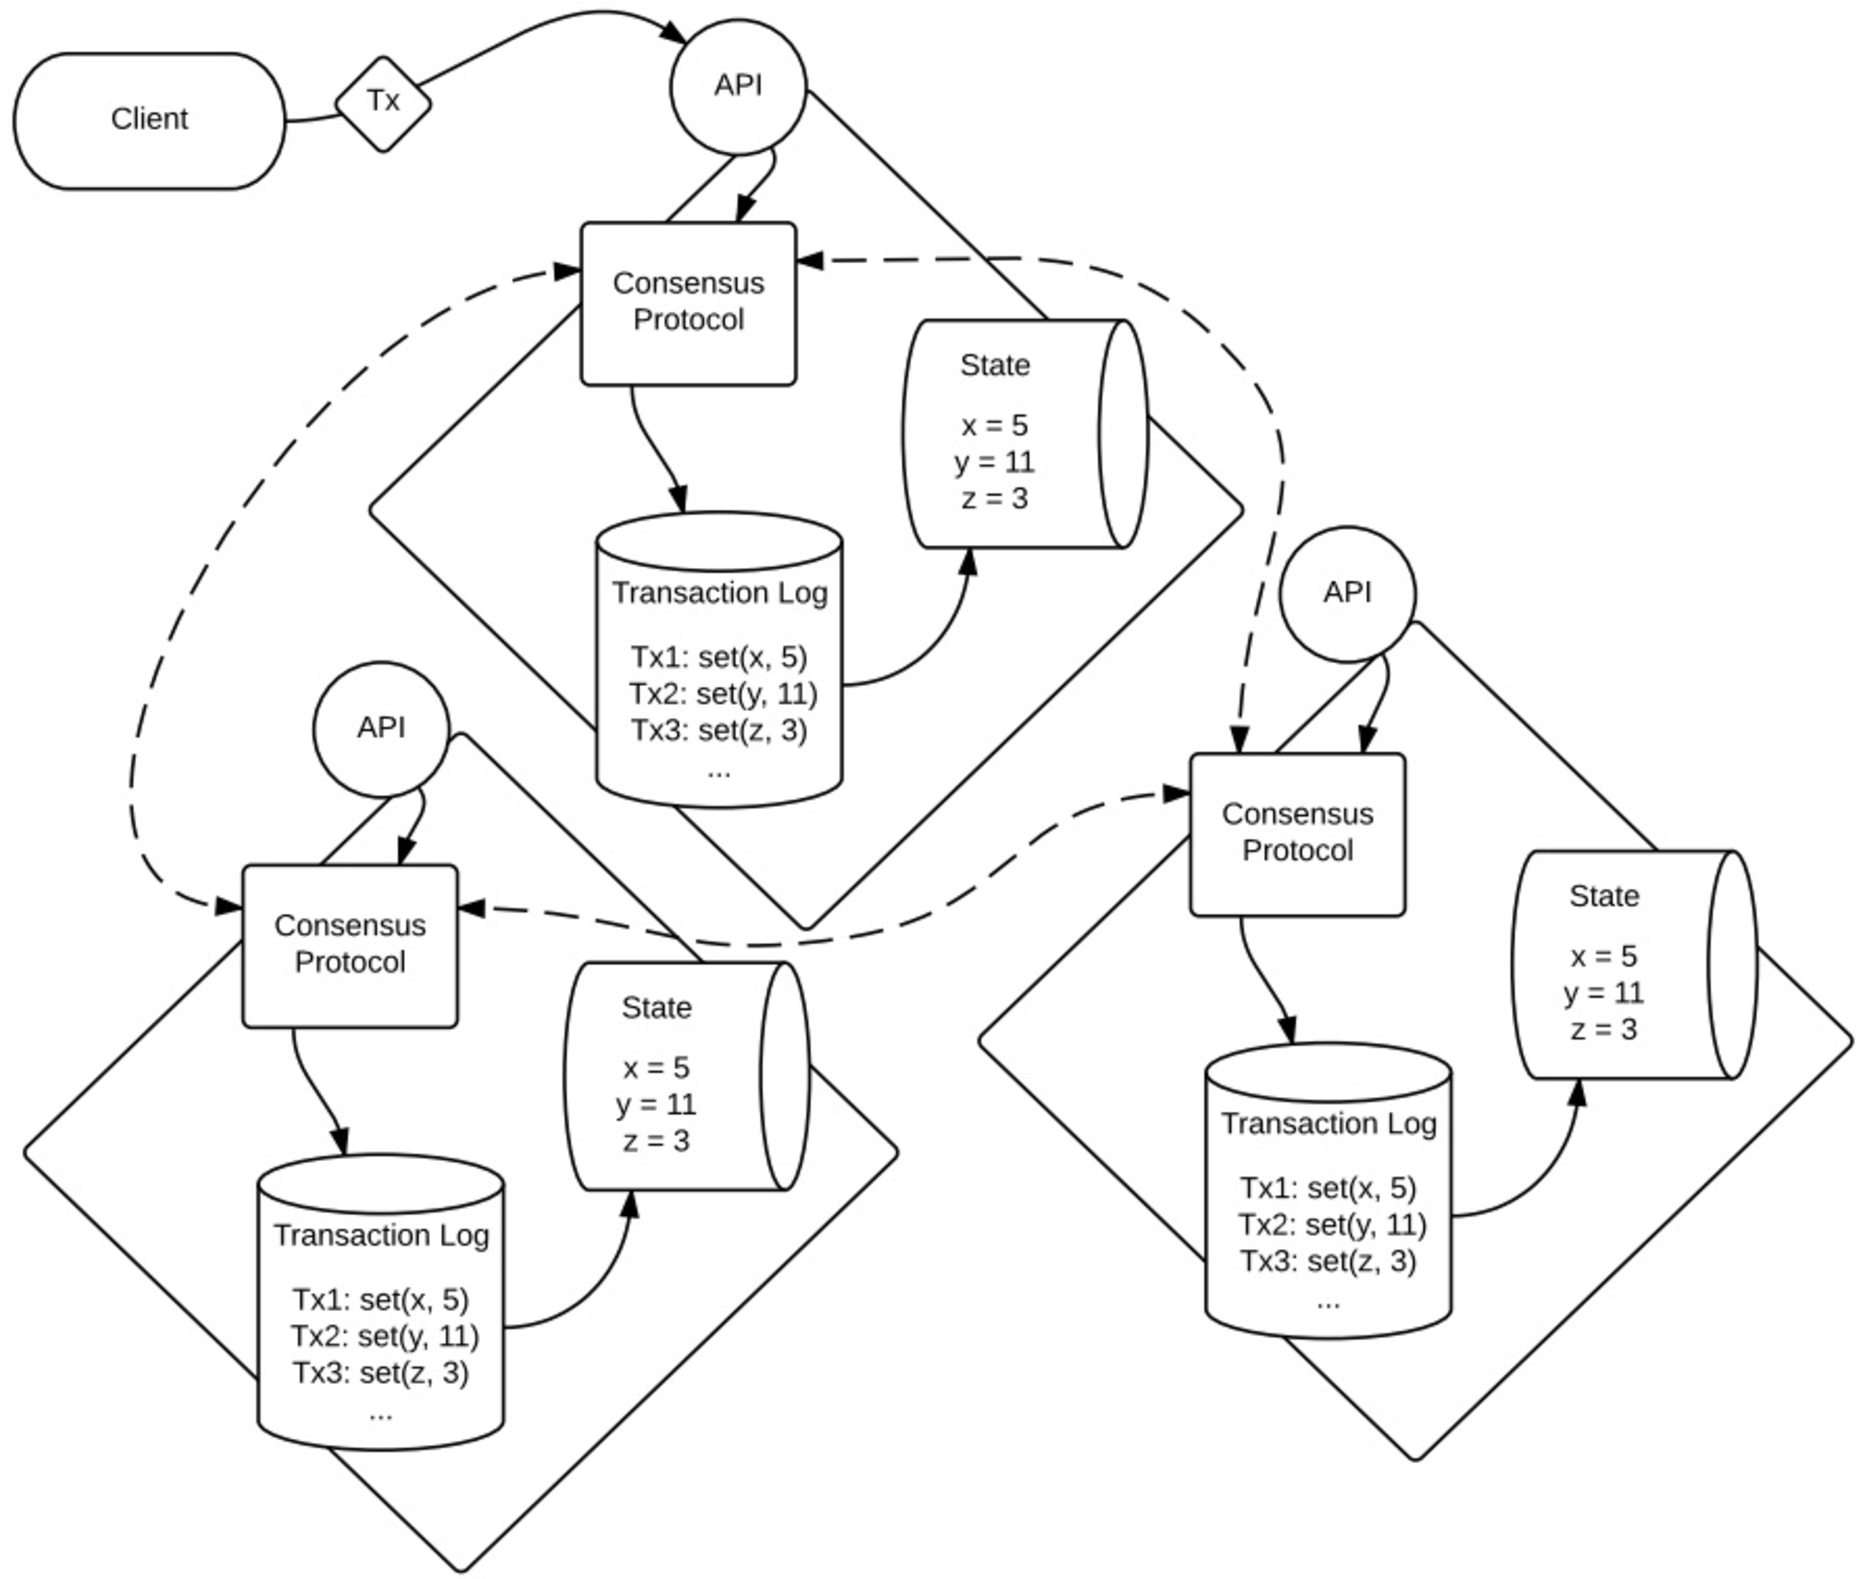
\includegraphics[scale=0.25]{figures/replication_engine.pdf}
  \caption{Overview of replicated state machine architecture~\cite{Buchman.2018.Tendermint}.
    %
    Diamonds represent machines.
    %
    Dotted lines represent communication between machines to carry out the
consensus protocol for ordering transactions
  }
  \label{fig:replication}
\end{figure}

%

Tendermint consists of two chief technical components: a blockchain consensus engine and a
generic application interface.
%
The consensus engine, called Tendermint Core, ensures that the same transactions are recorded
on every machine in the same order.
%
The application interface, called the Application BlockChain Interface (ABCI), enables the
transactions to be processed in any programming language.
%

\subsection{Application BlockChain Interface}
ABCI is the interface between Tendermint Core
% (the \textquotedblleft
% consensus engine\textquotedblright)
and the replicated application.
%
A Tendermint node maintains three main ABCI connections with the replicated application.
%

The \textit{consensus connection} is used only when a new block is committed,
and communicates all information from the block in a series of 
requests: \<BeginBlock>, [\<DeliverTx>, ...], \<EndBlock>, \<Commit>.
%
That is, when a block is committed in the consensus, Tendermint sends a 
list of \<DeliverTx> requests (one for each transaction) sandwiched by 
\<BeginBlock> and \<EndBlock> requests, and followed by a \<Commit>.

%

The \textit{mempool connection} is used by the transaction
pool protocol to validate transactions submitted
by clients against the application state. 
%
It is used only for \<CheckTx> requests. Transactions
are run using \<CheckTx> in the same order they were received
by the validator\footnote{Validator nodes are responsible for committing new blocks in the blockchain. These validators participate in the consensus protocol by broadcasting votes which contain cryptographic signatures signed by each validator's private key.}. If the \<CheckTx> returns OK, the transaction
is kept in memory and relayed to other peers in the same order
it was received. Otherwise, it is discarded.
%
It is up to the application to define whether a transaction is valid or not, and
the validation is optional. 

%

The \textit{query connection} allows retrieving information
from the local instance of the application, used by several
Tendermint modules (e.g., peer filtering).
%
It is used to query the application without engaging consensus. 
%It is exposed over the tendermint core rpc, so clients can query
%the app without exposing a server on the app itself.

Figure~\ref{fig:abci_flow} shows the flow of messages via consensus and mempool connections.
%

\begin{figure}
  \centering
  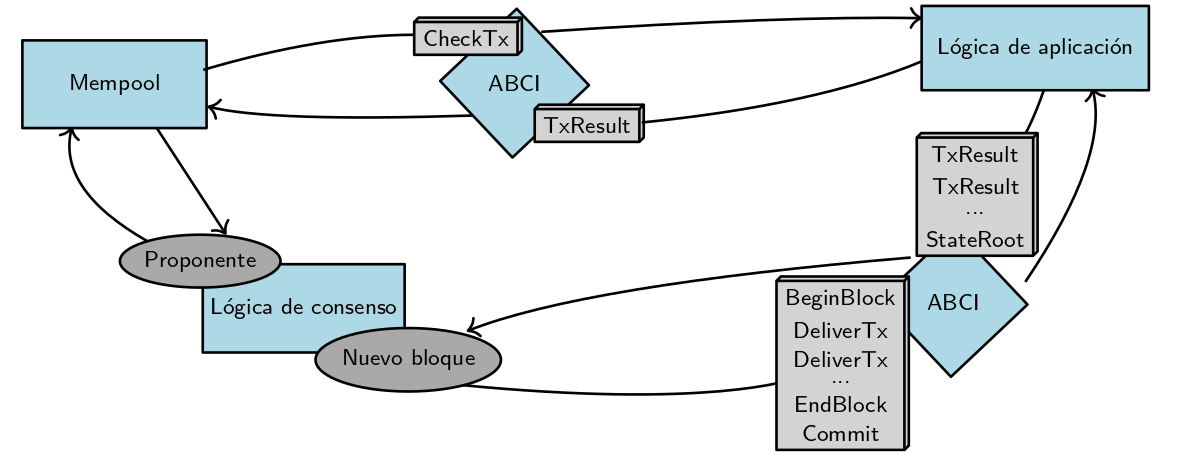
\includegraphics[scale=0.35]{figures/abci_msg_flow.pdf}
  \caption{Flow of messages via ABCI~\cite{tendermint.site}.}
  \label{fig:abci_flow}
\end{figure}

%%% Local Variables:
%%% TeX-master: "article.tex"
%%% TeX-PDF-mode: t
%%% End:
